\documentclass{article}

\usepackage{arxiv}

\usepackage[utf8]{inputenc} % allow utf-8 input
\usepackage[T1]{fontenc}    % use 8-bit T1 fonts
\usepackage{hyperref}       % hyperlinks
\usepackage{url}            % simple URL typesetting
\usepackage{booktabs}       % professional-quality tables
\usepackage{amsfonts}       % blackboard math symbols
\usepackage{nicefrac}       % compact symbols for 1/2, etc.
\usepackage{microtype}      % microtypography
\usepackage{graphicx}

\usepackage[numbers]{natbib}
\usepackage{amsmath,amssymb}
\usepackage{capt-of}
\usepackage[english]{babel}

\title{Early CNN Layer Homography and Feature-Space Augmentation for Training-Free Unaligned Industrial Anomaly Detection}

\author{
	Márk Király \\
	\texttt{mark.kiraly.hu@gmail.com}
}

\begin{document}
	\maketitle
	
	% Abstract
	\begin{abstract}
		Visual anomaly detectors currently have to choose between reliability tied to static environments and costly training, which, according to my observations, hinders their agile, High-Mix Low-Volume industrial application. As a potential solution to this problem, I propose OrbitCore, a training-free feature-space adaptation algorithm that integrates deep convolutional normalization, iterative homography registration performed on early layers, and feature-space statistical augmentation. Based on the results, my measurements on distorted data suggest that the method exhibits asymmetric behavior: alongside an increase in image-level robustness, filtering unstructured noise can globally improve localization accuracy, although I observed a loss of sensitivity for certain textures under sterile conditions. I believe the increased inference time resulting from iterative optimization can be an acceptable compromise for a purely decision-supporting industrial tool.
	\end{abstract}
	
	% Keywords
	\keywords{Visual Anomaly Detection \and Test-Time Adaptation \and Feature Alignment \and Pose Invariance \and Image Registration}
	
	% Main text
	\section{Introduction}\label{sec:intro}
	Standard solutions for industrial anomaly detection, such as PaDiM \cite{Defard2021} and PatchCore \cite{Roth2022}, assume static conditions and mechanically fixed camera views. In a real-world environment, slight changes in viewpoints and lighting differences can appear as false anomalies in the feature space, which can degrade classification reliability. This problem can be exponentially worse in agile, High-Mix Low-Volume (HMLV) manufacturing environments, where, due to the rapid change of product types and camera positions, no prior information is available about specific defect types, and training individual models does not prove to be a resource-efficient strategy. Although end-to-end fine-tuning of an invariant deep learning model could provide a solution, the continuous collection of data for new camera views and the computational costs associated with weight updating are often difficult to implement in practice. The goal of my current research is to investigate an approach that attempts to minimize geometric deviations between the static memory bank and the test sample during the test phase, without modifying the neural network parameters. I publish my implementation used for the experiments at the following link: \url{https://github.com/ProgrammerGnome/orbitcore_anomaly_detection}.
	
	\section{Related Work}\label{sec:related}
	\subsection{Deep Feature-Based SSAD}
	A significant portion of modern semi-supervised anomaly detection (SSAD) systems is based on deep representations extracted from convolutional networks pre-trained on large-scale natural image datasets. The literature discusses several notable trends, including reconstruction-based architectures (e.g., DRAEM \cite{Zavrtanik2021}), normalizing flows (e.g., CFLOW-AD \cite{Gudovskiy2022}), and knowledge distillation-based networks \cite{Deng2022}. Methods like PatchCore \cite{Roth2022} and PaDiM \cite{Defard2021} achieve good performance by modeling normal samples in a patch-level reference memory. Although recent extensions such as ReConPatch \cite{ReConPatch} and PatchCore-FR \cite{FRPatchCore} attempt to improve upon the base architectures, I opted not to rely on them, as they either introduce a computationally expensive training phase or still fundamentally rely on spatial determinism without explicitly resolving test-time geometric misalignments. However, these models rely on the assumption of spatial determinism. In a real industrial environment, however, according to my observations, objects frequently shift, which can lead to false anomaly signals for architectures built on static memory banks.
	
	\subsection{Image Registration and Homography}
	The classical approach to handling spatial deviations between visual observations is image registration \cite{Szeliski2006}. Traditional, keypoint-based methods rely on detecting local, high-contrast structures. In industrial environments, however, object surfaces are often homogeneous, where keypoint matching can become unreliable. Consequently, it seems appropriate to formulate the geometric alignment in a continuous representation space. Although the Spatial Transformer Network (STN) \cite{Jaderberg2015} would offer a differentiable alternative, the backbone network in industrial SSAD systems typically remains frozen to avoid overfitting. Thus, to the best of my knowledge, a strategy worth considering is deterministic, iterative optimization performed at test time.
	
	\subsection{Test-Time Adaptation}
	The test-time adaptation (TTA) paradigm addresses the problem where a model adapts to distribution shifts during the test phase \cite{Sun2020}. Classical TTA approaches typically rely on partially updating the neural network parameters. My proposal, OrbitCore, in contrast, is a training-free test-time adaptation experiment. Instead of modifying the network weights, I optimize the geometry of the input representation in the deep feature space using an iterative procedure.
	
	\subsection{Feature-Space Augmentation and Aggregation}
	To increase prediction robustness, averaging multiple transformed versions of the input images at the output is a long-used practice \cite{Krizhevsky2012}. At the same time, modern research has moved towards performing augmentation within the continuous and dense convolutional feature space itself to protect against distribution shifts \cite{Upadhyay2022}. In my OrbitCore approach, I adapt this concept for memory bank-based detection.
	
	\section{Methodology}
	\subsection{Deterministic Feature Extraction and Photometric Normalization}
	\label{subsec:feature_extraction}
	As a starting point, I consider an input image $X \in \mathbb{R}^{3 \times H_0 \times W_0}$. A pre-trained convolutional network with frozen weights (e.g., ResNet-18 \cite{He2016}) generates hierarchical feature maps. To avoid task-specific overfitting and preserve spatial resolution, I use the outputs of the middle layers (layer 2 and layer 3), which I bring to the same resolution using bilinear interpolation, and then concatenate along the channel dimension to obtain the raw tensor $\hat{f}_{raw} \in \mathbb{R}^{C \times H \times W}$.
	
	In an industrial environment, the dynamic change in lighting appears as local intensity scaling in the input image space. Passing through convolutional networks, this effect can cause a drastic change in the magnitude of feature vectors. Since memory bank-based SSAD models rely on Euclidean distance measurement, preserving high-dimensional concatenated tensors would lead to severe memory bottlenecks. Before any photometric stabilization, I reduce the channel dimensions of $\hat{f}_{raw}$ to a fixed target dimension ($C_{target} = 128$) using a deterministic Sparse Random Projection (SRP) matrix. 
	
	Subsequently, to eliminate the effect of dynamic lighting, I apply channel-wise $L_2$ normalization at every spatial position $(x, y)$ in the OrbitCore model:
	\begin{equation}
		f_{norm}(c, x, y) = \frac{\hat{f}_{raw}(c, x, y)}{\sqrt{\sum_{k=1}^C \hat{f}_{raw}(k, x, y)^2 + \epsilon}}
	\end{equation}
	where $\epsilon = 10^{-5}$ ensures numerical stability. In my view, this operation increases photometric invariance. The anomaly search is henceforth based on the angles subtended by the vectors (cosine distances). To increase position-independent robustness, I calculate a local mean ($\mu$) and standard deviation ($\sigma$) with a kernel size of $K \times K$, and then concatenate them for the final base representation: $\phi = [\mu, \sigma]$.
	
	\subsection{Feature-Space Homography}
	\label{subsec:homography}
	I try to minimize the distortions originating from uncalibrated viewpoints iteratively, isolated from the training phase. Crucially, to preserve deep semantic structures and reduce computational overhead, this test-time adaptation (TTA) is not applied to the final fused representation. Instead, I perform the homography registration explicitly on the early, low-level spatial features extracted from the first residual block (Layer 1). Let $f_{1, test}$ denote this early test feature map, and $f_{1, ref}$ the reference. In a practical HMLV setup, finding an ideal anchor point is challenging. Therefore, OrbitCore deterministically records the early layer features of the very first nominal sample during the training phase to serve as a global spatial reference ($f_{1, ref}$) for all subsequent test-time alignments. I model the geometric relation with a $3 \times 3$ projective transformation matrix $H(\mathbf{p})$:
	\begin{equation}
		H(\mathbf{p}) = \begin{bmatrix} 1 + p_1 & p_2 & p_3 \\ p_4 & 1 + p_5 & p_6 \\ p_7 & p_8 & 1 \end{bmatrix}
	\end{equation}
	
	The goal of the test-time adaptation (TTA), in my view, is to find $\mathbf{p}^*$ that maximizes structural similarity through an adapted inverse loss function of the Enhanced Correlation Coefficient (ECC) \cite{Evangelidis2008}. However, geometric alignment on the high-resolution deep feature space raises a non-convex optimization problem.
	
	To avoid this, I reduce the feature maps to a radically downscaled $8 \times 8$ grid and flatten the channels into vectors $\mathbf{v}_{test, c}$ and $\mathbf{v}_{ref, c}$ before loss calculation:
	\begin{equation}
		\mathcal{L}_{ECC}(\mathbf{p}) = 1 - \frac{1}{C} \sum_{c=1}^C \frac{\mathbf{v}_{test, c}^T \mathbf{v}_{ref, c}}{\|\mathbf{v}_{test, c}\|_2 \|\mathbf{v}_{ref, c}\|_2}
	\end{equation}
	According to my observations, this dimension reduction can act as a spatial low-pass filter, suppressing textural noise. I perform the optimization iteratively, isolated from the training phase (Algorithm 1), using the Adam algorithm. By compensating for scale differences, Adam can ensure more stable convergence even during the tested narrow (e.g., $max\_iter=60$) iteration timeframe, which I illustrate in Figure \ref{fig:convergence}.
	
	\begin{center}
		\nopagebreak
		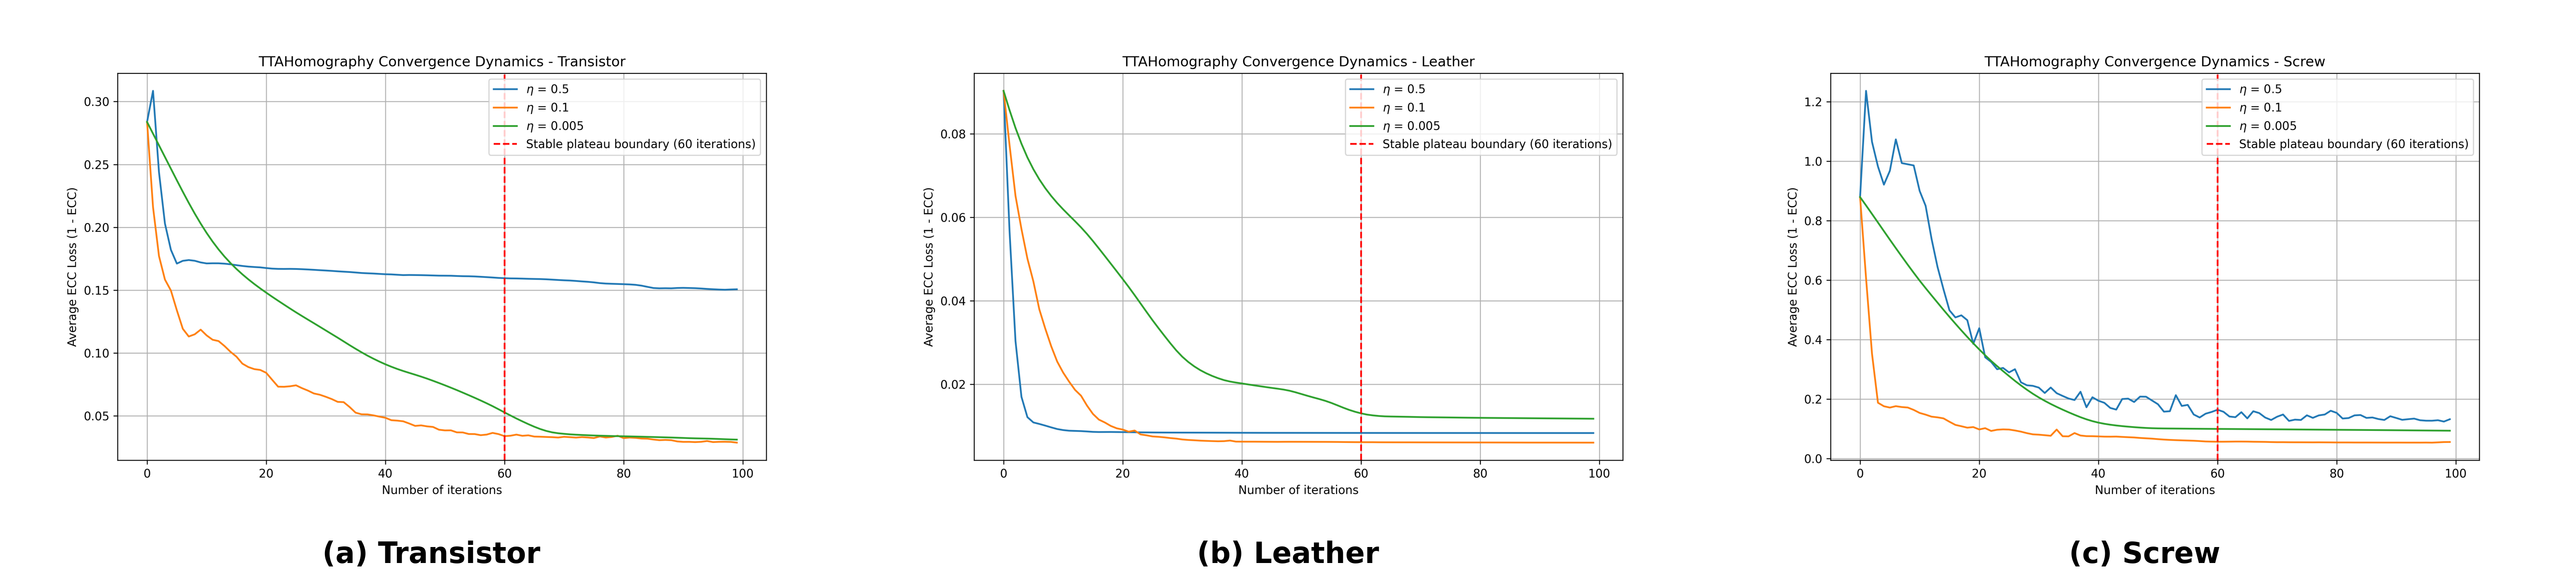
\includegraphics[width=0.9\linewidth, height=0.35\textheight, keepaspectratio]{convergence.png}
		\captionof{figure}{\textbf{Convergence during the specified iterations.} Based on the measurements, the Adam optimizer typically reaches a stable plateau within 60 iterations on the presented objects.}
		\label{fig:convergence}
	\end{center}
	
	% Pseudo-code block for Homography
	\begin{table}[h]
		\centering
		\begin{tabular}{l}
			\toprule
			\textbf{Algorithm 1} Feature-Space Homography Optimization \\
			\midrule
			\textbf{Input:} $\phi_{test}$, $\phi_{ref}$, max\_iter $= 100$, $\eta = 0.1$ \\
			\textbf{Init:} $\mathbf{p} \leftarrow \mathbf{0} \in \mathbb{R}^8$ (requires\_grad = True) \\
			\textbf{Optimizer:} Adam($[\mathbf{p}]$, lr=$\eta$) \\
			1: \textbf{for} $i = 1$ \textbf{to} max\_iter \textbf{do} \\
			2: \quad Optimizer.zero\_grad() \\
			3: \quad Grid $\leftarrow$ CreateHomographyGrid($\mathbf{p}$, height, width) \\
			4: \quad $\phi_{warp} \leftarrow$ BilinearSample($\phi_{test}$, Grid) \\
			5: \quad Loss $\leftarrow \mathcal{L}_{ECC}(\phi_{warp}, \phi_{ref})$ \\
			6: \quad Loss.backward() \\
			7: \quad Optimizer.step() \\
			8: \textbf{end for} \\
			\textbf{Output:} $\phi_{aligned} = \text{BilinearSample}(\phi_{test}, \text{Grid}(\mathbf{p}^*))$ \\
			\bottomrule
		\end{tabular}
	\end{table}
	
	To ensure that the localized anomalies accurately correspond to the original, unaligned physical space, the calculated geometric shift $\mathbf{p}^*$ is preserved. After calculating the final anomaly heatmaps in the aligned feature space, an inverse homography transformation is applied to map the predictions back to the original coordinates of the test sample.
	
	\subsection{Feature-Space Averaging}
	\label{subsec:orbit_averaging}
	Following deterministic image registration, microscopic interpolation errors may remain. To compensate for this, OrbitCore generates a fixed statistical framework on the registered feature map. I define 5 discrete projective perturbations for the perspective components of the parameter space $\mathbf{p}$, using a radius $\alpha$. In order to avoid invariance-based overfitting, I aligned the value of $\alpha$ to the expected maximum physical camera displacement ($\alpha = 0.3$). The elements of the transformation set are:
	\begin{equation}
		\mathcal{P}_{orbit} = \left\{ \mathbf{0}, [0 \dots \alpha, 0]^T, [0 \dots -\alpha, 0]^T, [0 \dots 0, \alpha]^T, [0 \dots 0, -\alpha]^T \right\}
	\end{equation}
	With each perturbation, I generate the shifted feature map. The final representation is the average of these states, supplemented with the standard deviation. Crucially, this statistical aggregation is applied during both the training and inference phases, ensuring that the reference memory bank itself is populated with robust, orbit-averaged representations.
	
	\begin{center}
		\nopagebreak
		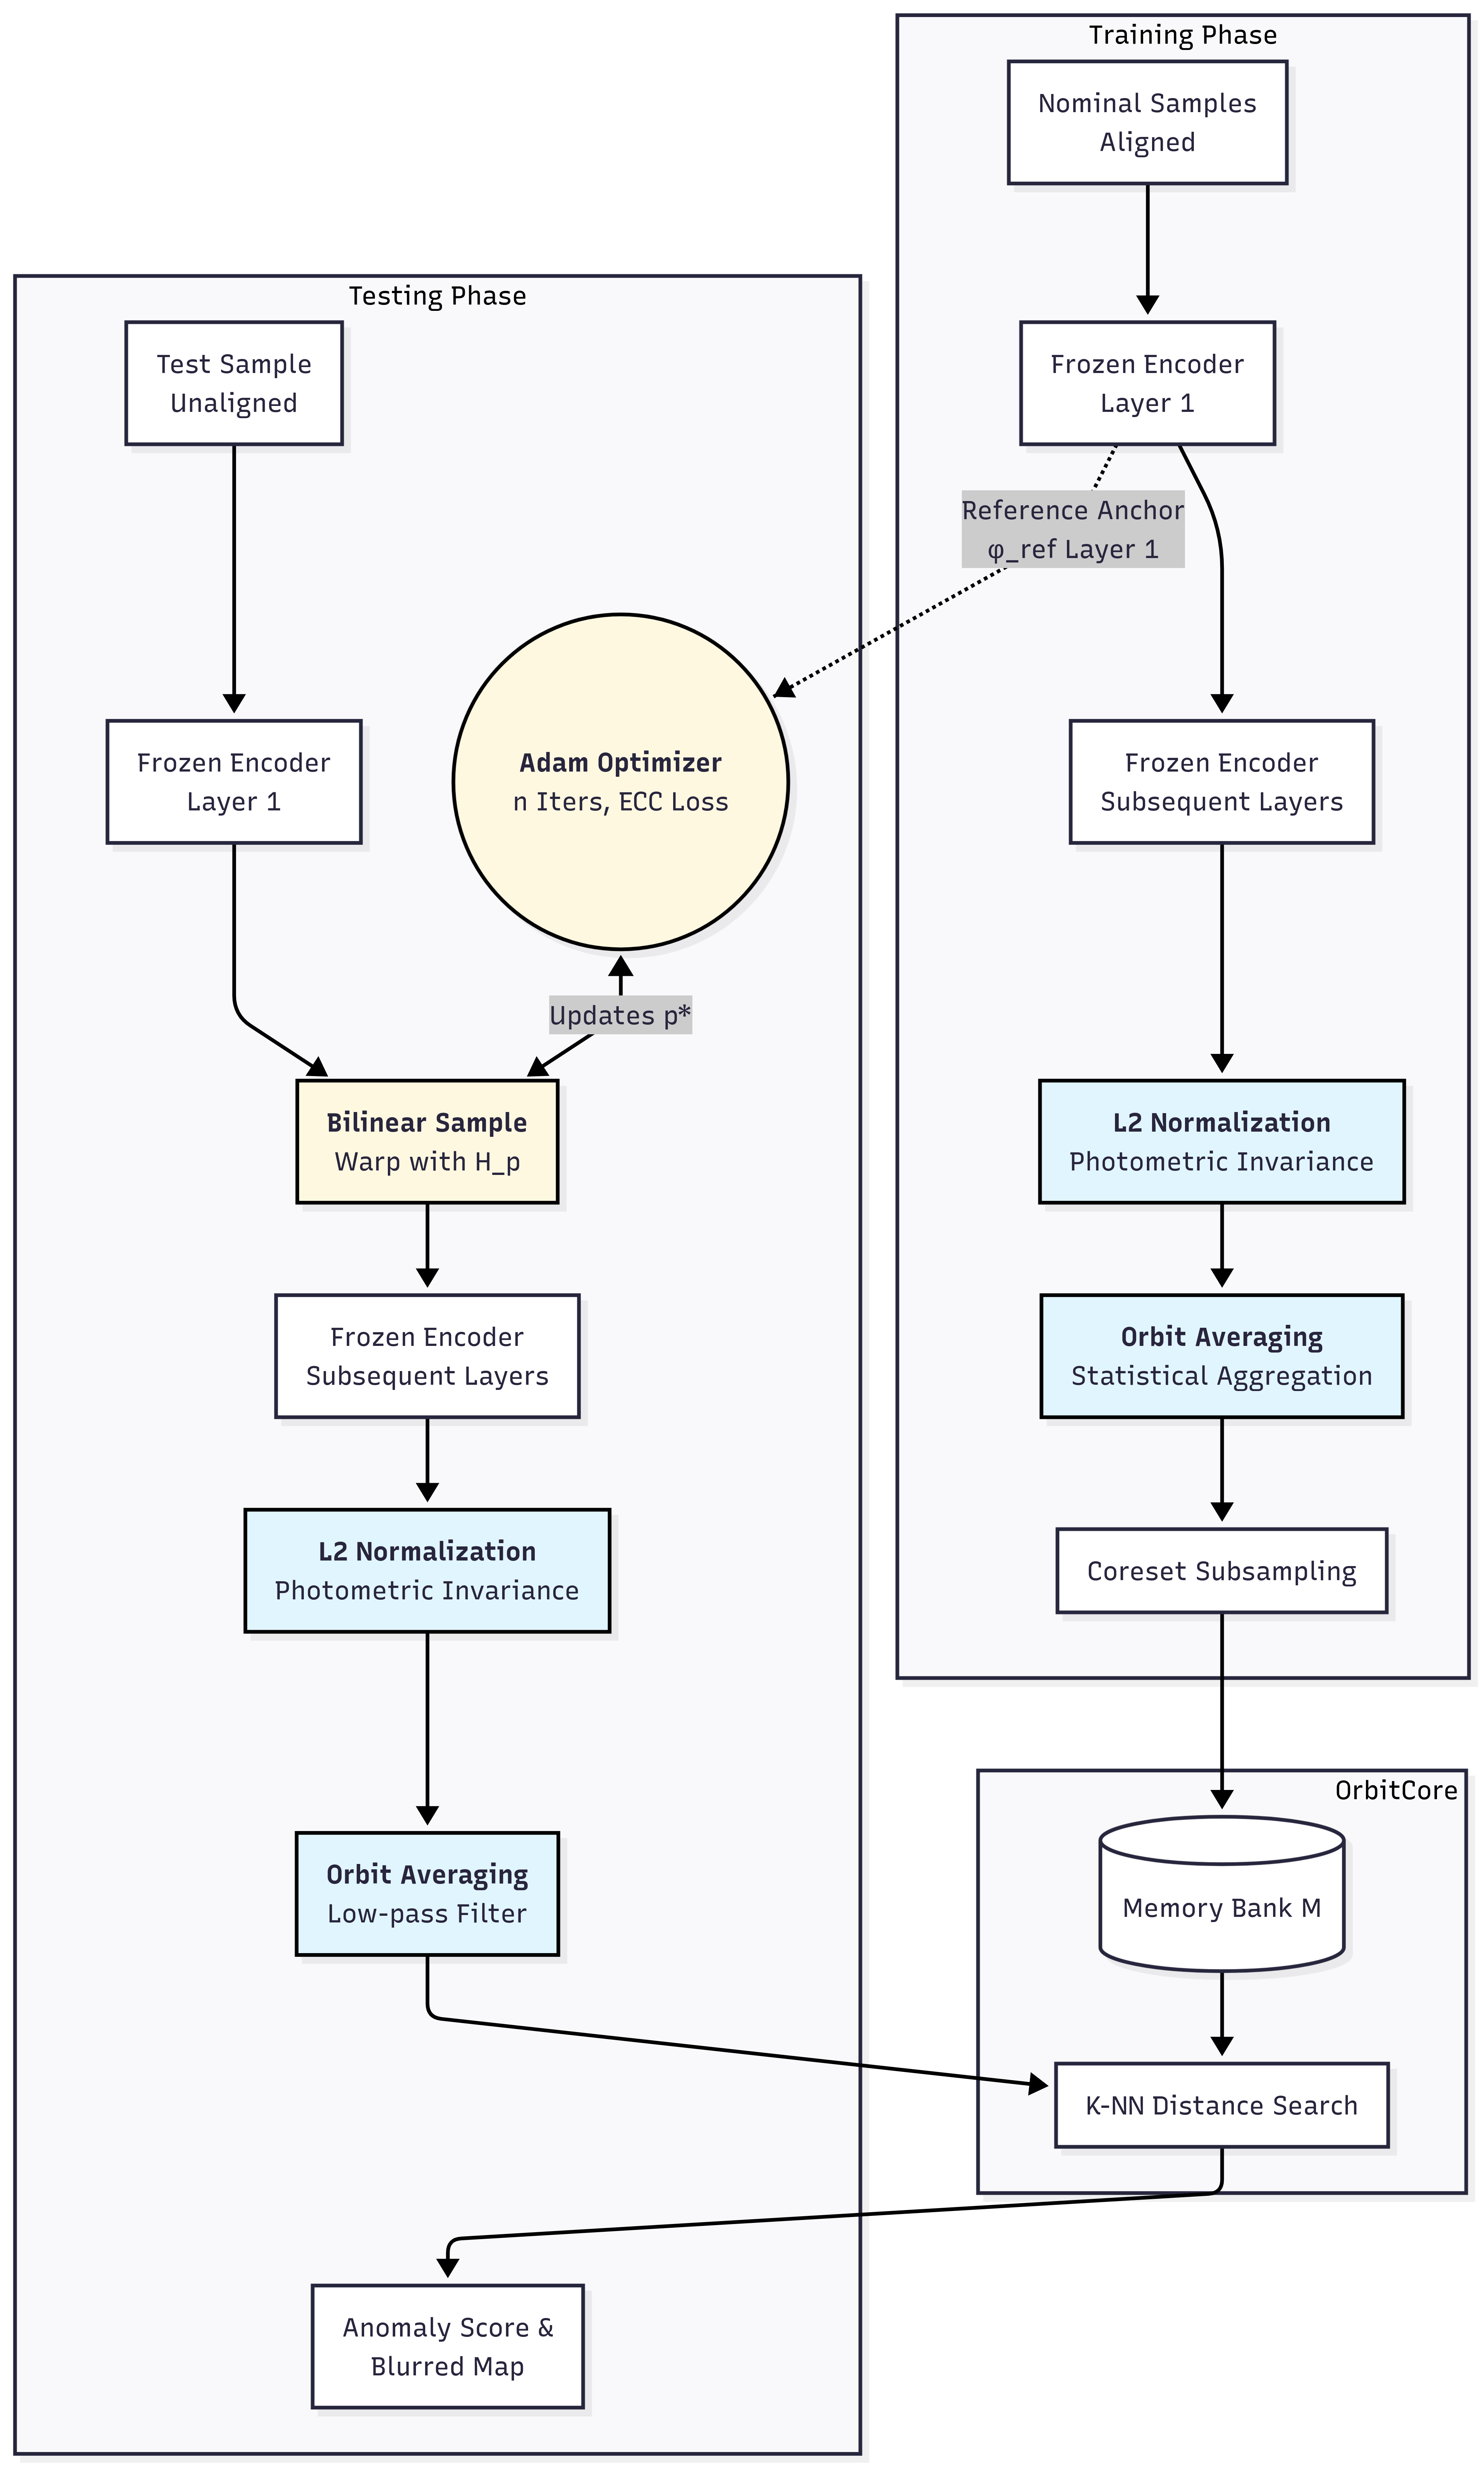
\includegraphics[width=1.0\linewidth, height=0.45\textheight, keepaspectratio]{orbitcore.png}
		\captionof{figure}{\textbf{Methodological overview of OrbitCore.} The flowchart summarizes the steps of iterative homography registration and feature-space augmentation.}
		\label{fig:method_overview}
	\end{center}
	
	\section{Experimental Protocol}
	\label{sec:experimental_setup}
	During the experimental validation, I used the PaDiM \cite{Defard2021} and PatchCore \cite{Roth2022} architectures as references. Selecting these models was a conscious methodological decision: similar to my approach, they do not require neural network training \cite{FRPatchCore}. In my judgment, this can provide a clearer picture of the effectiveness of algorithmic adaptation and feature-space averaging.
	
	\subsection{Dataset and Preprocessing}
	I performed the evaluation on the MVTec AD dataset \cite{Bergmann2019}. For training, I used the 3629 flawless samples, while the evaluation took place on the 1725 test images. I resized every image to a resolution of $256 \times 256$ pixels, then normalized them with ImageNet statistics. To simulate industrial uncalibration, I generated synthetic distortion boundary conditions on the test set.
	
	\subsection{Selection of Evaluation Metrics}
	To measure the performance of the models, I strictly applied the Area Under the Receiver Operating Characteristic Curve (AUROC) metric. Although the F1-score is common in industrial practice, in my view, its application in static memory bank SSAD research can lead to methodological biases due to arbitrary threshold selection.
	
	\subsection{Compensation for Receptive Field Distortion}
	In order to attribute the performance degradation of the baseline models purely to geometric incompatibility as much as possible, I introduced an experimental protocol: during the training phase, I applied a 16-pixel-wide black border to the reference images so that the models learn to tolerate the presence of boundary edges. Additionally, to analytically suppress false positives arising from grid-sample border padding during homography, a strict 2-pixel wide zero-masking is applied to the outermost edges of the predicted anomaly maps.
	
	\subsection{Implementation Details and Complexity}
	I ran all measurements in an NVIDIA Tesla T4 GPU environment. I fixed the hyperparameters of OrbitCore based on heuristics ($\eta = 0.1$, $iter = 100$, $\alpha = 0.3$).
	
	\textbf{Avoiding the Invariance Paradox:} If I tuned the geometric tolerance exclusively on the validation set, the model might interpret true anomalies as nominal textures due to an excessively large tolerance radius. To avoid this, I applied the $\alpha = 0.3$ heuristic.
	
	\textbf{Algorithmic Complexity:} OrbitCore supplements standard K-NN distance measurement with iterative optimization. Since I perform the optimization on a drastically reduced grid ($8 \times 8$), the additional cost can remain asymptotically manageable.
	
	\section{Results and Discussion}\label{sec:results}
	
	\subsection{Degradation of Static Models}
	I examine the evaluation results at two resolution levels, where Figure \ref{fig:robustness} contextualizes the problem as a function of distortion levels. During the experimental protocol, I defined four transformation boundary conditions of building intensity for the systematic analysis of the extent of distribution shift. The baseline is represented by the Level 0 (Clean) level, which measures the nominal performance of the models under distortion-free, sterile conditions. This is followed by the Level 1 (Micro) level, which introduces mild perturbations—$\pm 1^\circ$ rotation, $1\%$ translation, and a $0.1$ perspective scale—simulating finer mechanical inaccuracies. Increasing the degree of distortion, the Level 2 (Standard) level already represents moderate shifts ($\pm 2^\circ$ rotation, $2\%$ translation, $0.2$ scale), while the Level 3 (Extreme) configuration tests the invariance of the algorithms with drastic geometric deviations ($\pm 5^\circ$ rotation, $5\%$ translation, $0.4$ scale).
	
	Based on the measurement data, it appears that static memory banks struggle with significant functional difficulties even at the smallest geometric deviations (Level 1), which can be attributed to the violation of spatial determinism. In contrast, according to my observations, OrbitCore (Feature TTA) suffers a significantly more moderate OOD degradation; although its accuracy shown on sterile data may fall short of specialized static models, its performance stabilizes as distortion levels rise, and in my view, it offers a more robust alternative in variable industrial environments.
	
	\begin{center}
		\nopagebreak
		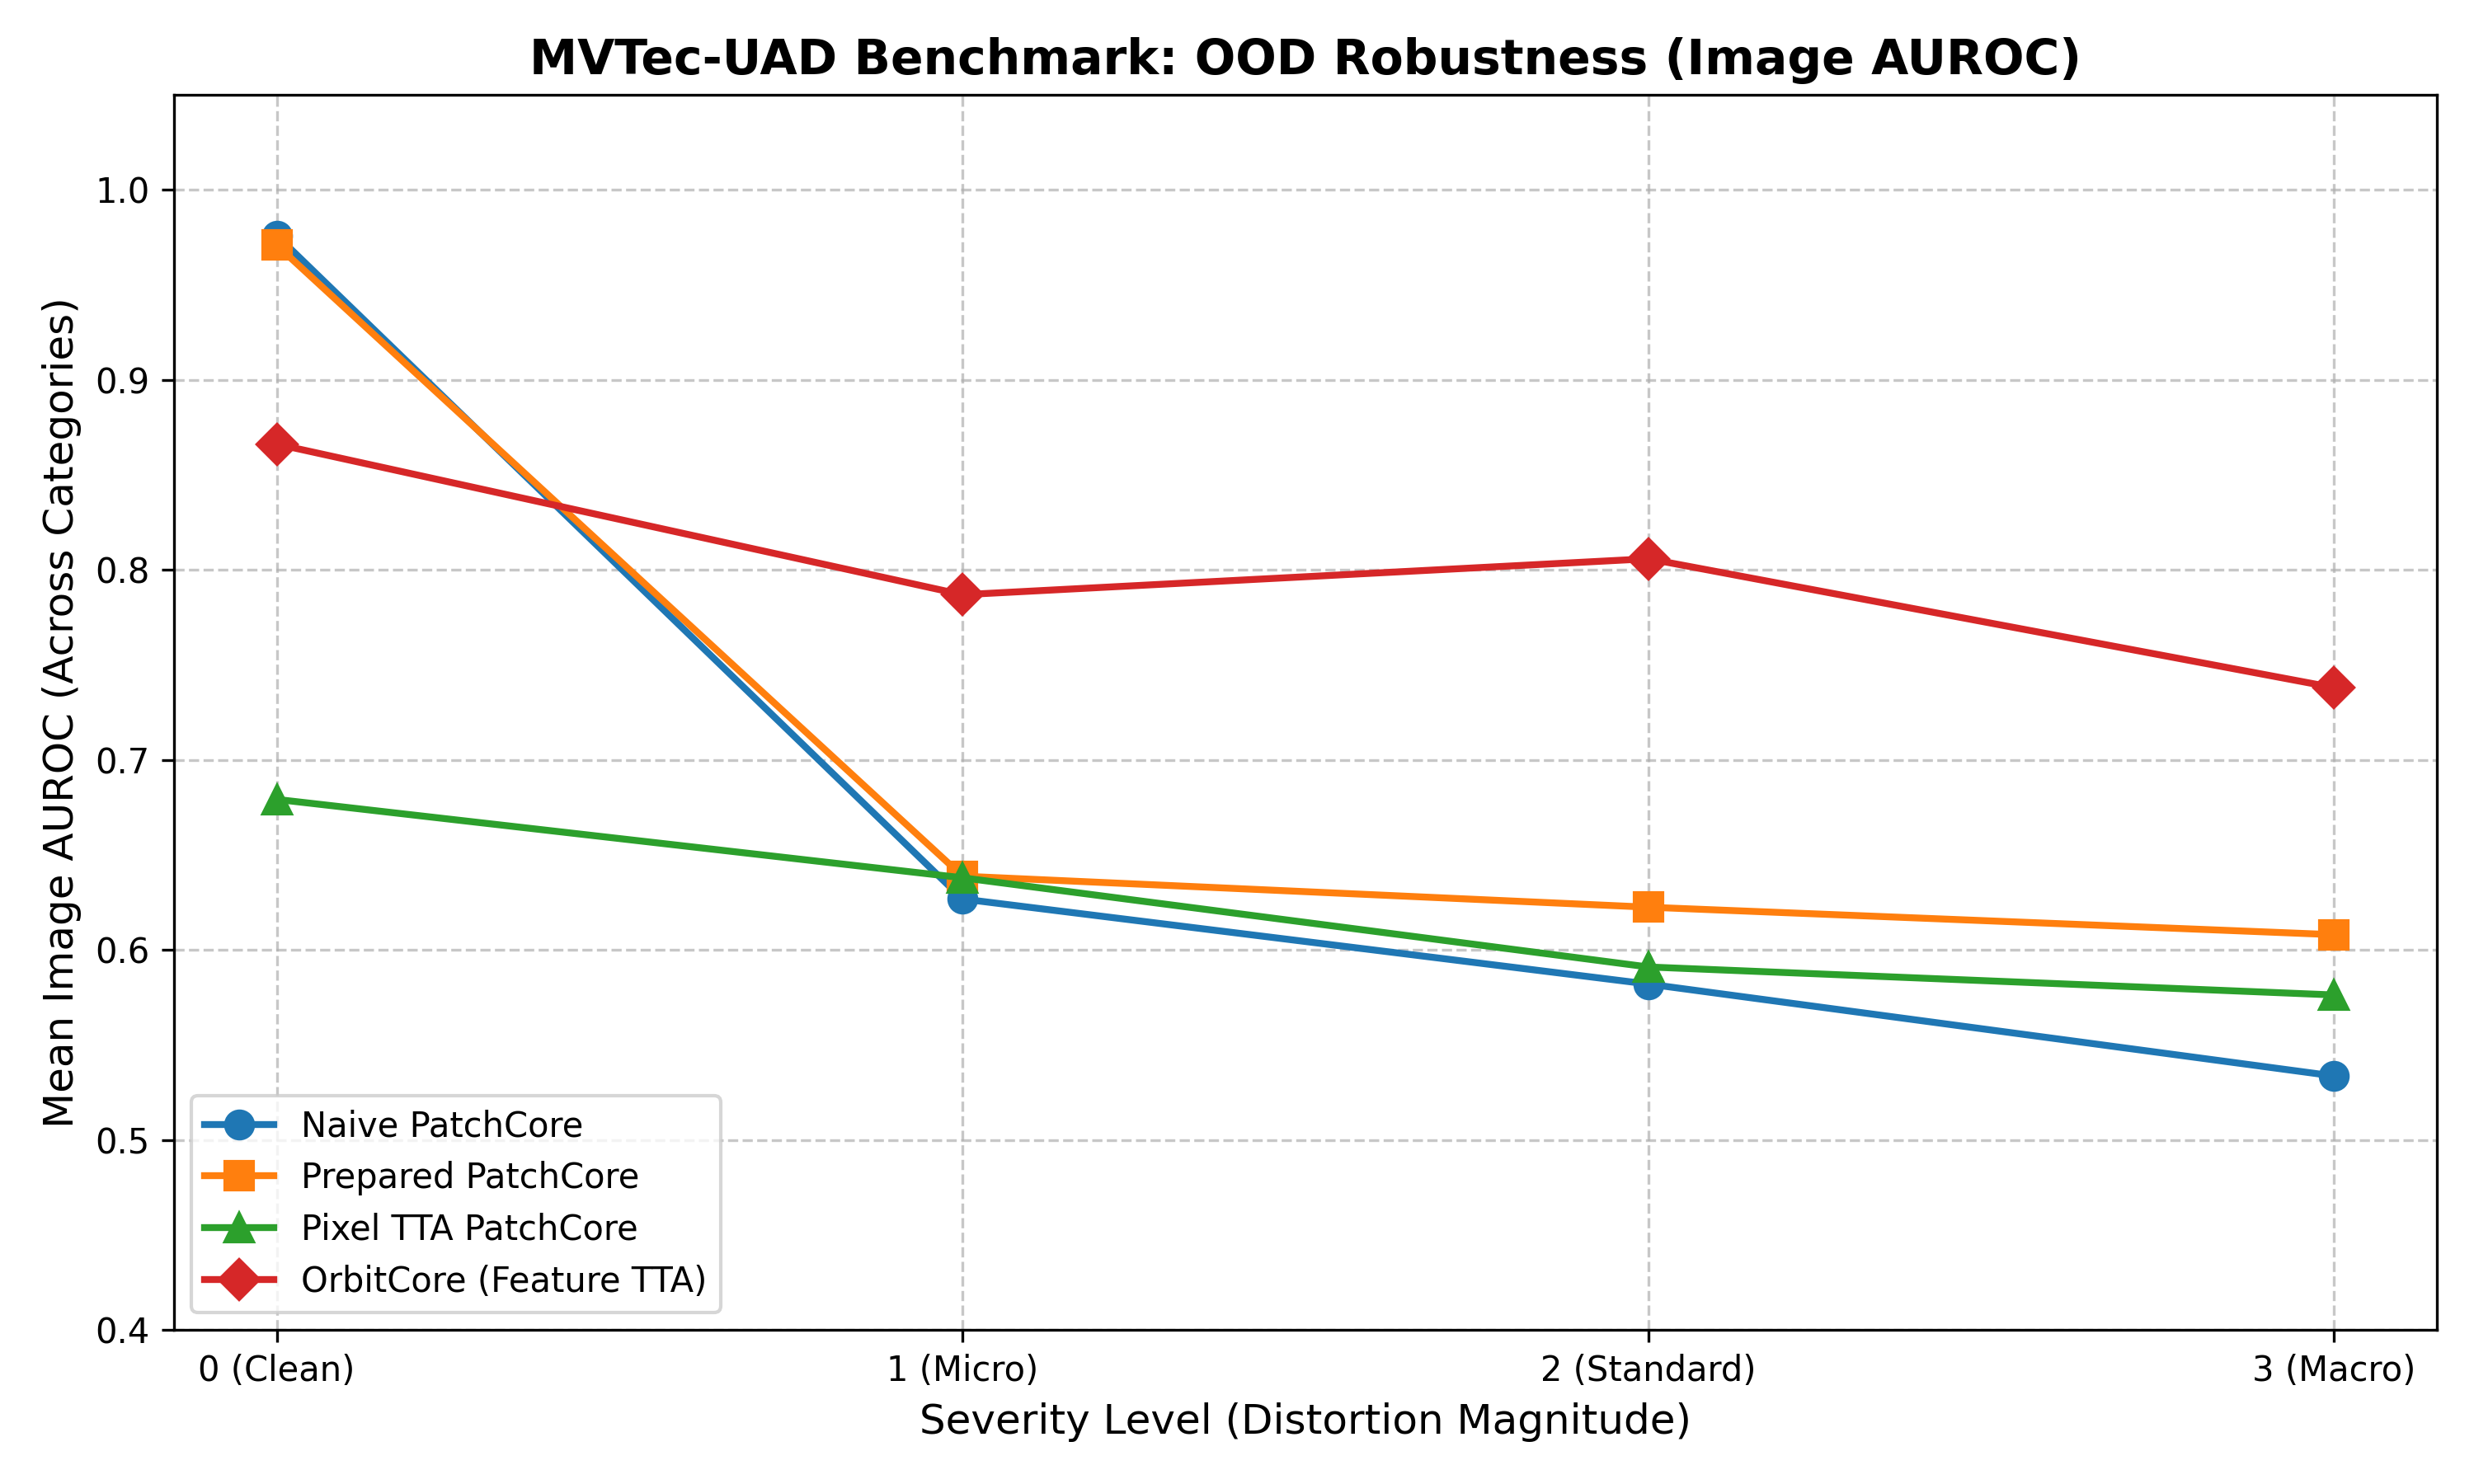
\includegraphics[width=0.9\linewidth, height=0.2\textheight, keepaspectratio]{mvtec_uad_robustness_plot.png}
		\captionof{figure}{Degradation Benchmark on the distorted MVTec AD dataset. Based on my measurements, static models can suffer performance loss due to distortions, while OrbitCore remained more stable in the examined cases.}
		\label{fig:robustness}
	\end{center}
	
	The results of the macro-level evaluation are presented in Table \ref{tbl:full_results}.
	
	\begin{table}[t]
		\centering
		\caption{Results of MVTec AD categories on the distorted dataset. Format: Image AUROC / Pixel AUROC. Best values are in bold.}\label{tbl:full_results}
		
		% 1. BLOKK: Objektumok (1-5)
		\begin{tabular}{@{} l ccccc @{}}
			\toprule
			\textbf{Architecture} & \textbf{Bottle} & \textbf{Cable} & \textbf{Capsule} & \textbf{Hazelnut} & \textbf{Metal Nut} \\
			\midrule
			1. Naive PaDiM & 0.502 / 0.642 & 0.462 / 0.648 & 0.509 / 0.689 & 0.519 / 0.719 & 0.442 / 0.692 \\
			2. PaDiM + Pixel TTA & 0.487 / 0.867 & 0.545 / 0.828 & 0.491 / 0.842 & 0.555 / 0.707 & 0.430 / 0.732 \\
			3. Prepared PaDiM & 0.471 / 0.551 & 0.476 / 0.584 & 0.500 / 0.593 & 0.500 / 0.601 & 0.524 / 0.626 \\
			4. Naive PatchCore & 0.489 / 0.828 & 0.562 / 0.915 & 0.518 / 0.695 & 0.644 / 0.938 & 0.724 / 0.950 \\
			5. PatchCore + Pixel TTA & 0.884 / 0.959 & 0.515 / 0.926 & 0.541 / 0.863 & 0.646 / 0.916 & 0.829 / 0.958 \\
			6. Prepared PatchCore & 0.409 / 0.759 & 0.574 / 0.871 & 0.483 / 0.607 & 0.668 / 0.938 & 0.833 / \textbf{0.962} \\
			7. Pixel TTA (No Orbit) & 0.829 / 0.912 & 0.689 / 0.895 & 0.497 / 0.854 & 0.446 / 0.786 & 0.806 / 0.908 \\
			8. Feature TTA (No Orbit) & 0.930 / 0.955 & 0.780 / 0.941 & 0.630 / 0.809 & 0.789 / 0.871 & 0.724 / 0.888 \\
			9. Orbit (No TTA) & 0.842 / 0.798 & 0.616 / 0.836 & 0.491 / 0.548 & 0.934 / 0.934 & \textbf{0.896} / 0.891 \\
			10. OrbitCore (Pixel TTA) & 0.941 / 0.933 & 0.833 / 0.942 & 0.517 / 0.836 & 0.754 / 0.876 & 0.856 / 0.952 \\
			11. OrbitCore (Feature TTA)& \textbf{0.976} / \textbf{0.969} & \textbf{0.939} / \textbf{0.962} & \textbf{0.647} / \textbf{0.869} & \textbf{0.959} / \textbf{0.949} & 0.890 / 0.929 \\
			\bottomrule
		\end{tabular}
		
		\vspace{1.5em}
		
		% 2. BLOKK: Objektumok (6-10)
		\begin{tabular}{@{} l ccccc @{}}
			\toprule
			\textbf{Architecture} & \textbf{Pill} & \textbf{Screw} & \textbf{Toothbrush} & \textbf{Transistor} & \textbf{Zipper} \\
			\midrule
			1. Naive PaDiM & 0.597 / 0.550 & 0.592 / \textbf{0.779} & 0.647 / 0.864 & 0.553 / 0.677 & 0.425 / 0.695 \\
			2. PaDiM + Pixel TTA & 0.495 / 0.807 & 0.477 / 0.627 & 0.590 / 0.908 & 0.548 / 0.554 & 0.531 / 0.497 \\
			3. Prepared PaDiM & 0.617 / 0.506 & 0.580 / 0.656 & 0.647 / 0.849 & 0.592 / 0.616 & 0.435 / 0.633 \\
			4. Naive PatchCore & 0.592 / 0.860 & \textbf{0.649} / 0.739 & \textbf{0.817} / \textbf{0.967} & 0.507 / 0.795 & 0.607 / 0.724 \\
			5. PatchCore + Pixel TTA & 0.681 / \textbf{0.934} & 0.459 / 0.629 & 0.700 / 0.955 & 0.536 / 0.582 & 0.383 / 0.498 \\
			6. Prepared PatchCore & 0.693 / 0.929 & 0.644 / 0.640 & 0.797 / \textbf{0.967} & 0.491 / 0.747 & 0.404 / 0.624 \\
			7. Pixel TTA (No Orbit) & 0.560 / 0.844 & 0.457 / 0.579 & 0.560 / 0.910 & 0.613 / 0.574 & 0.467 / 0.498 \\
			8. Feature TTA (No Orbit) & 0.528 / 0.896 & 0.501 / 0.739 & 0.710 / 0.916 & 0.950 / 0.895 & \textbf{0.846} / 0.614 \\
			9. Orbit (No TTA) & 0.556 / 0.754 & 0.648 / 0.564 & 0.736 / 0.881 & 0.652 / 0.863 & 0.438 / \textbf{0.731} \\
			10. OrbitCore (Pixel TTA) & 0.675 / 0.881 & 0.471 / 0.572 & 0.596 / 0.941 & 0.613 / 0.577 & 0.487 / 0.492 \\
			11. OrbitCore (Feature TTA)& \textbf{0.737} / 0.915 & 0.512 / 0.758 & 0.761 / 0.960 & \textbf{0.987} / \textbf{0.954} & 0.841 / 0.613 \\
			\bottomrule
		\end{tabular}
		
		\vspace{1.5em}
		
		% 3. BLOKK: Textúrák (1-5)
		\begin{tabular}{@{} l ccccc @{}}
			\toprule
			\textbf{Architecture} & \textbf{Carpet} & \textbf{Grid} & \textbf{Leather} & \textbf{Tile} & \textbf{Wood} \\
			\midrule
			1. Naive PaDiM & 0.551 / 0.887 & 0.444 / 0.668 & 0.681 / 0.924 & 0.620 / 0.741 & 0.683 / 0.813 \\
			2. PaDiM + Pixel TTA & 0.493 / 0.558 & 0.437 / 0.558 & 0.545 / 0.519 & 0.602 / 0.538 & 0.732 / 0.521 \\
			3. Prepared PaDiM & 0.576 / 0.856 & 0.476 / 0.590 & 0.705 / 0.879 & 0.553 / 0.664 & 0.607 / 0.723 \\
			4. Naive PatchCore & 0.467 / 0.867 & 0.429 / 0.694 & 0.554 / 0.906 & 0.495 / 0.755 & 0.536 / 0.774 \\
			5. PatchCore + Pixel TTA & 0.511 / 0.586 & 0.465 / 0.555 & 0.552 / 0.519 & 0.536 / 0.537 & 0.633 / 0.520 \\
			6. Prepared PatchCore & 0.658 / \textbf{0.932} & 0.444 / 0.681 & 0.712 / 0.893 & 0.458 / 0.711 & 0.443 / 0.724 \\
			7. Pixel TTA (No Orbit) & 0.645 / 0.597 & 0.430 / 0.572 & 0.503 / 0.521 & 0.494 / 0.595 & 0.656 / 0.542 \\
			8. Feature TTA (No Orbit) & 0.626 / 0.815 & \textbf{0.742} / \textbf{0.750} & \textbf{0.852} / 0.674 & 0.805 / 0.689 & 0.805 / 0.760 \\
			9. Orbit (No TTA) & 0.504 / 0.832 & 0.457 / 0.633 & 0.818 / \textbf{0.971} & 0.633 / \textbf{0.773} & 0.705 / \textbf{0.815} \\
			10. OrbitCore (Pixel TTA) & 0.645 / 0.602 & 0.430 / 0.572 & 0.503 / 0.521 & 0.496 / 0.593 & 0.728 / 0.542 \\
			11. OrbitCore (Feature TTA)& \textbf{0.748} / 0.830 & 0.706 / 0.742 & 0.846 / 0.660 & \textbf{0.839} / 0.689 & \textbf{0.857} / 0.762 \\
			\bottomrule
		\end{tabular}
	\end{table}
	
	\subsection{Ablation Study on the Synergy of Components}
	I analyze the individual contribution of each component of the proposed method within an ablation study in rows 7-11 of Table \ref{tbl:full_results}. In my view, the configuration based purely on Orbit averaging (row 9: Orbit (No TTA)) alone can mostly only compensate for minimal distortions, whereas purely feature-space homography (row 8: Feature TTA (No Orbit)) effectively handles macro-geometric deviations, but can remain sensitive to interpolation noise. The results may suggest that the integration of the two approaches (row 11: OrbitCore (Feature TTA)) results in a synergistic effect that can simultaneously mitigate both types of errors, significantly increasing robustness compared to partial solutions. Furthermore, the comparison between pixel-level alignment performed in the raw image space (Pixel TTA) and continuous feature-space alignment (Feature TTA) seems to confirm the assumption that in the context of industrial anomaly detection, registration performed in the deep, normalized space can be more effective.
	
	Based on the above measurements, OrbitCore also produced asymmetric, texture-dependent results. The local loss of sensitivity (e.g., in the leather category), in my opinion, could be the failure of spatial registration. Excessively homogeneous textures presumably do not provide enough structural anchor points for optimization.
	
	I also subjected the macro-level analysis to a statistical test (10 iterations $\pm$ standard deviation) in Table \ref{tbl:stat_results}, based on which the results can be considered significant ($p < 0.05$) in the affected categories.
	
	\begin{table}[h]
		\centering
		\caption{Statistical significance test (Image AUROC \%) based on the mean and standard deviation of 10 independent runs.}
		\label{tbl:stat_results}
		\begin{tabular}{lccc}
			\toprule
			\textbf{Category} & \textbf{Naive PatchCore} & \textbf{OrbitCore (Ours)} & \textbf{p-value} \\
			\midrule
			Transistor & $51,73 \pm 6,25$ & $\mathbf{91,65 \pm 3,68}$ & $< 0,00001$ \\
			Leather    & $56,50 \pm 5,62$ & $\mathbf{77,79 \pm 3,78}$ & $< 0,00001$ \\
			Screw      & $\mathbf{66,06 \pm 2,64}$ & $52,42 \pm 5,89$ & $0,00002$ \\
			\bottomrule
		\end{tabular}
	\end{table}
	
	\begin{figure}[t]
		\centering
		\includegraphics[width=0.9\textwidth]{heatmaps_comparison.png}
		\caption{Qualitative comparison of the heatmaps of static and adaptive models on distorted inputs. Columns: (a) Distorted RGB image; (b) Original RGB image; (c) Naive PatchCore prediction; (d) OrbitCore (Ours) prediction. \textbf{Top row:} Successful registration on a structured object according to my observation. \textbf{Bottom row:} Geometric alignment failure on a homogeneous texture, where the lack of proper anchor points led to an incorrect alignment.}
		\label{fig:heatmaps}
	\end{figure}
	
	\subsection{Boundary Artifacts vs. Real Defect}
	The control masking introduced during the experiment (Prepared PatchCore), based on my observations, did not yield the expected robustness against test-time shifts. In contrast, OrbitCore's feature-space registration (Figure \ref{fig:heatmaps}d) can analytically compensate for spatial asymmetry.
	
	\subsection{Inference Latency}
	While standard PatchCore's inference time averages $0.13 - 0.34$ seconds/batch, iterative optimization increases this to $0.17 - 0.41$ seconds according to my observations. I believe that the processing speed of $\sim 2-5$ frames per second can still satisfy the requirements of certain industrial quality control tasks.
	
	\section{Conclusion}\label{sec:conclusion}
	Based on the results, I believe that OrbitCore, through early feature-space geometric registration, can contribute to improving the decision-making capability of memory bank-based anomaly detectors shown in uncalibrated environments. According to my observations, the experiments may suggest that the method can reduce false anomalies arising from macro-geometric deviations. However, the theoretical limitation of the procedure seems clear to me: in the case of homogeneous, repeating textures, geometric alignment can become uncertain in the absence of anchor points. Furthermore, in my opinion, it might be worthwhile in the future to test the experiment discussed in the article on a dataset containing real images, created specifically for this purpose, instead of synthetic data.
	
	%\newpage
	
	%% Loading bibliography style file
	\bibliographystyle{unsrt}
	
	% Loading bibliography database
	\bibliography{cas-refs}
	
\end{document}